\chapter{Improved porosimetric techniques for highly ultramicroporous carbons}
\label{ch:dual_isotherm}

\section{Introduction}

\section{Initial dual isotherm analyses}

\newpage
\section[Publication II]{Publication II: Confirmation of pore formation mechanisms in biochars and activated carbons by dual isotherm analysis}

\textbf{Contribution of the author}: The author performed all synthesis and instrumental analysis of samples in the work, analysed the results and wrote the manuscript.

\newpage

\setlength{\originalVOffset}{\voffset}   
\setlength{\originalHOffset}{\hoffset}

\setlength{\voffset}{0cm}
\setlength{\hoffset}{0cm}
%add pdf later
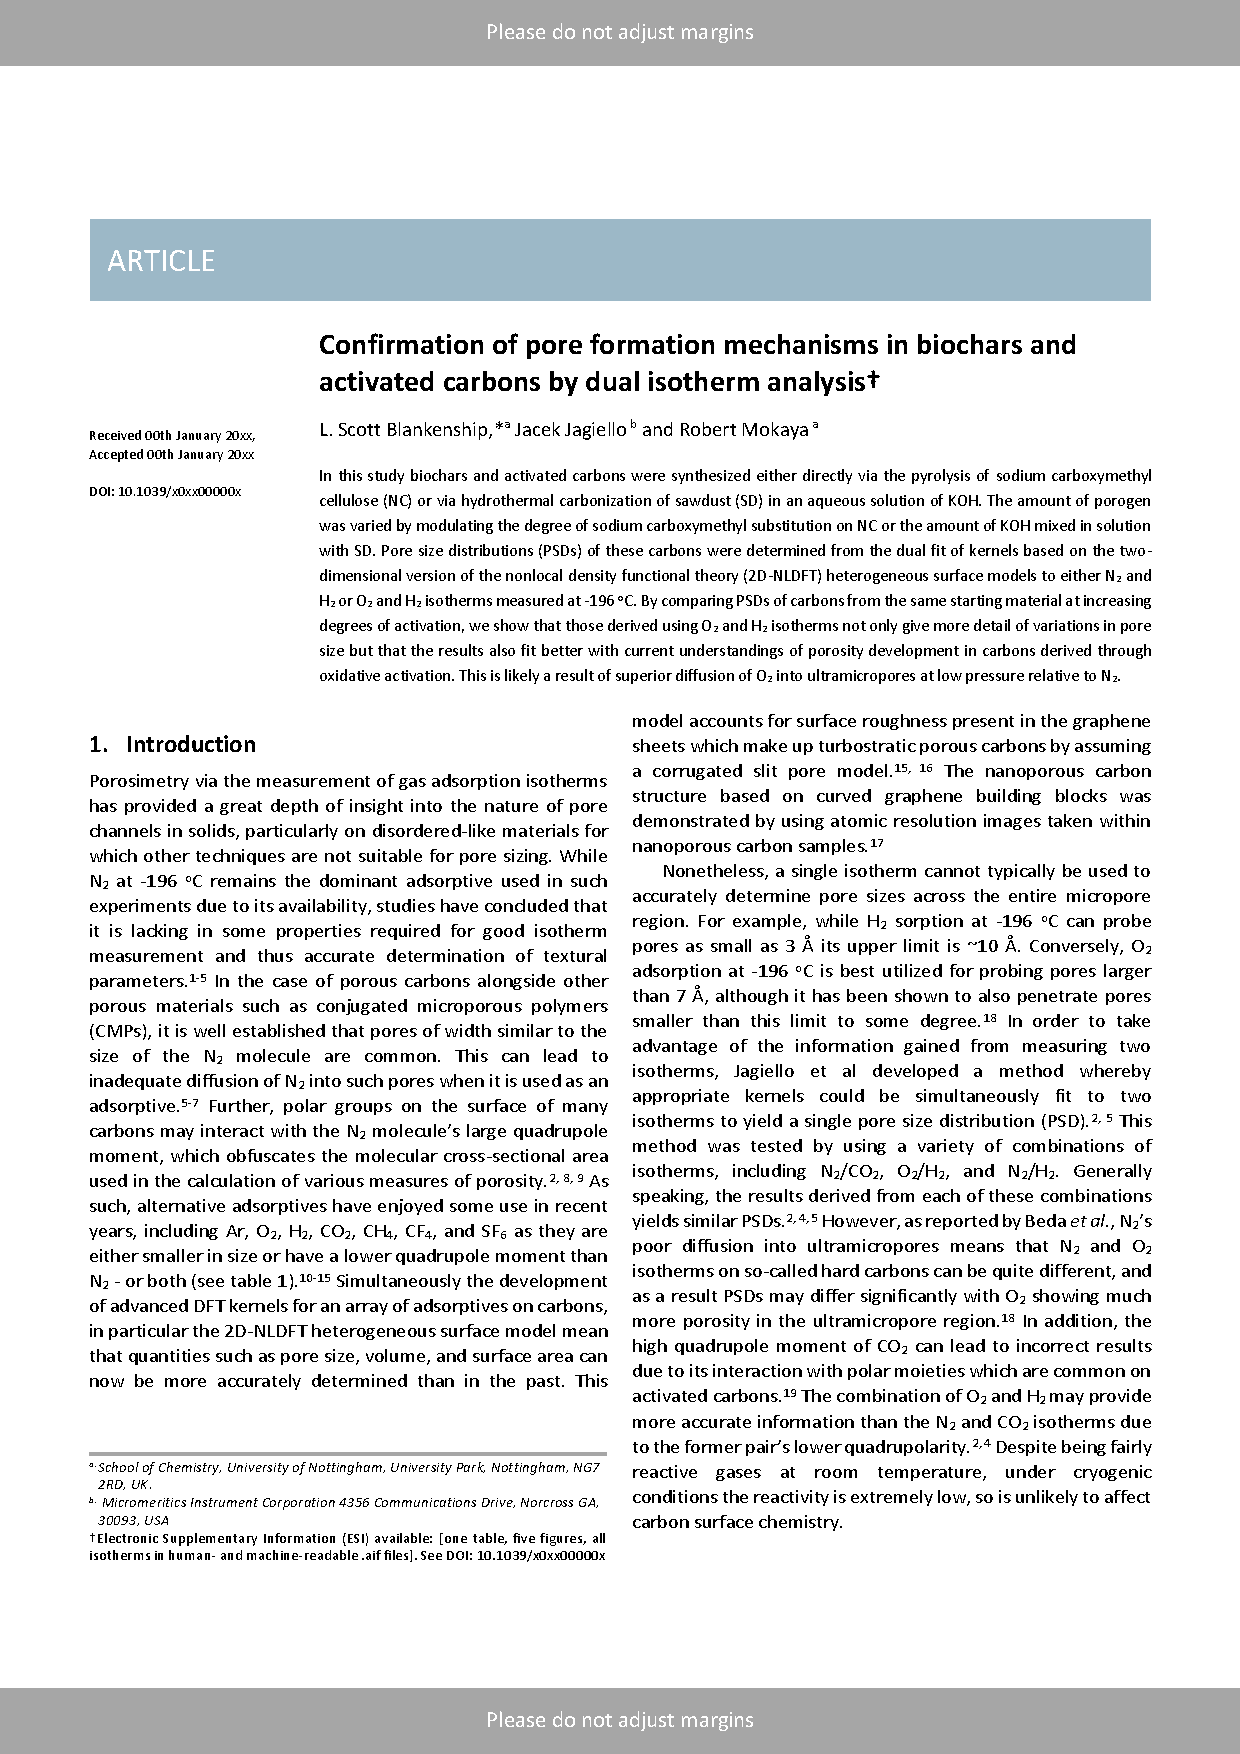
\includepdf[pages=-]{publication_02}
\setlength{\voffset}{\originalVOffset}
\setlength{\hoffset}{\originalHOffset}

\section{Results \& Discussion}
\subsection{Single isotherm}
\subsection{Dual isotherm}

\newpage
\section[Publication II Supporting Information]{Publication II Supporting Information: Confirmation of pore formation mechanisms in biochars and activated carbons by dual isotherm analysis}


\newpage

\setlength{\originalVOffset}{\voffset}   
\setlength{\originalHOffset}{\hoffset}

\setlength{\voffset}{0cm}
\setlength{\hoffset}{0cm}
% too big for overleaf, try compilation later.
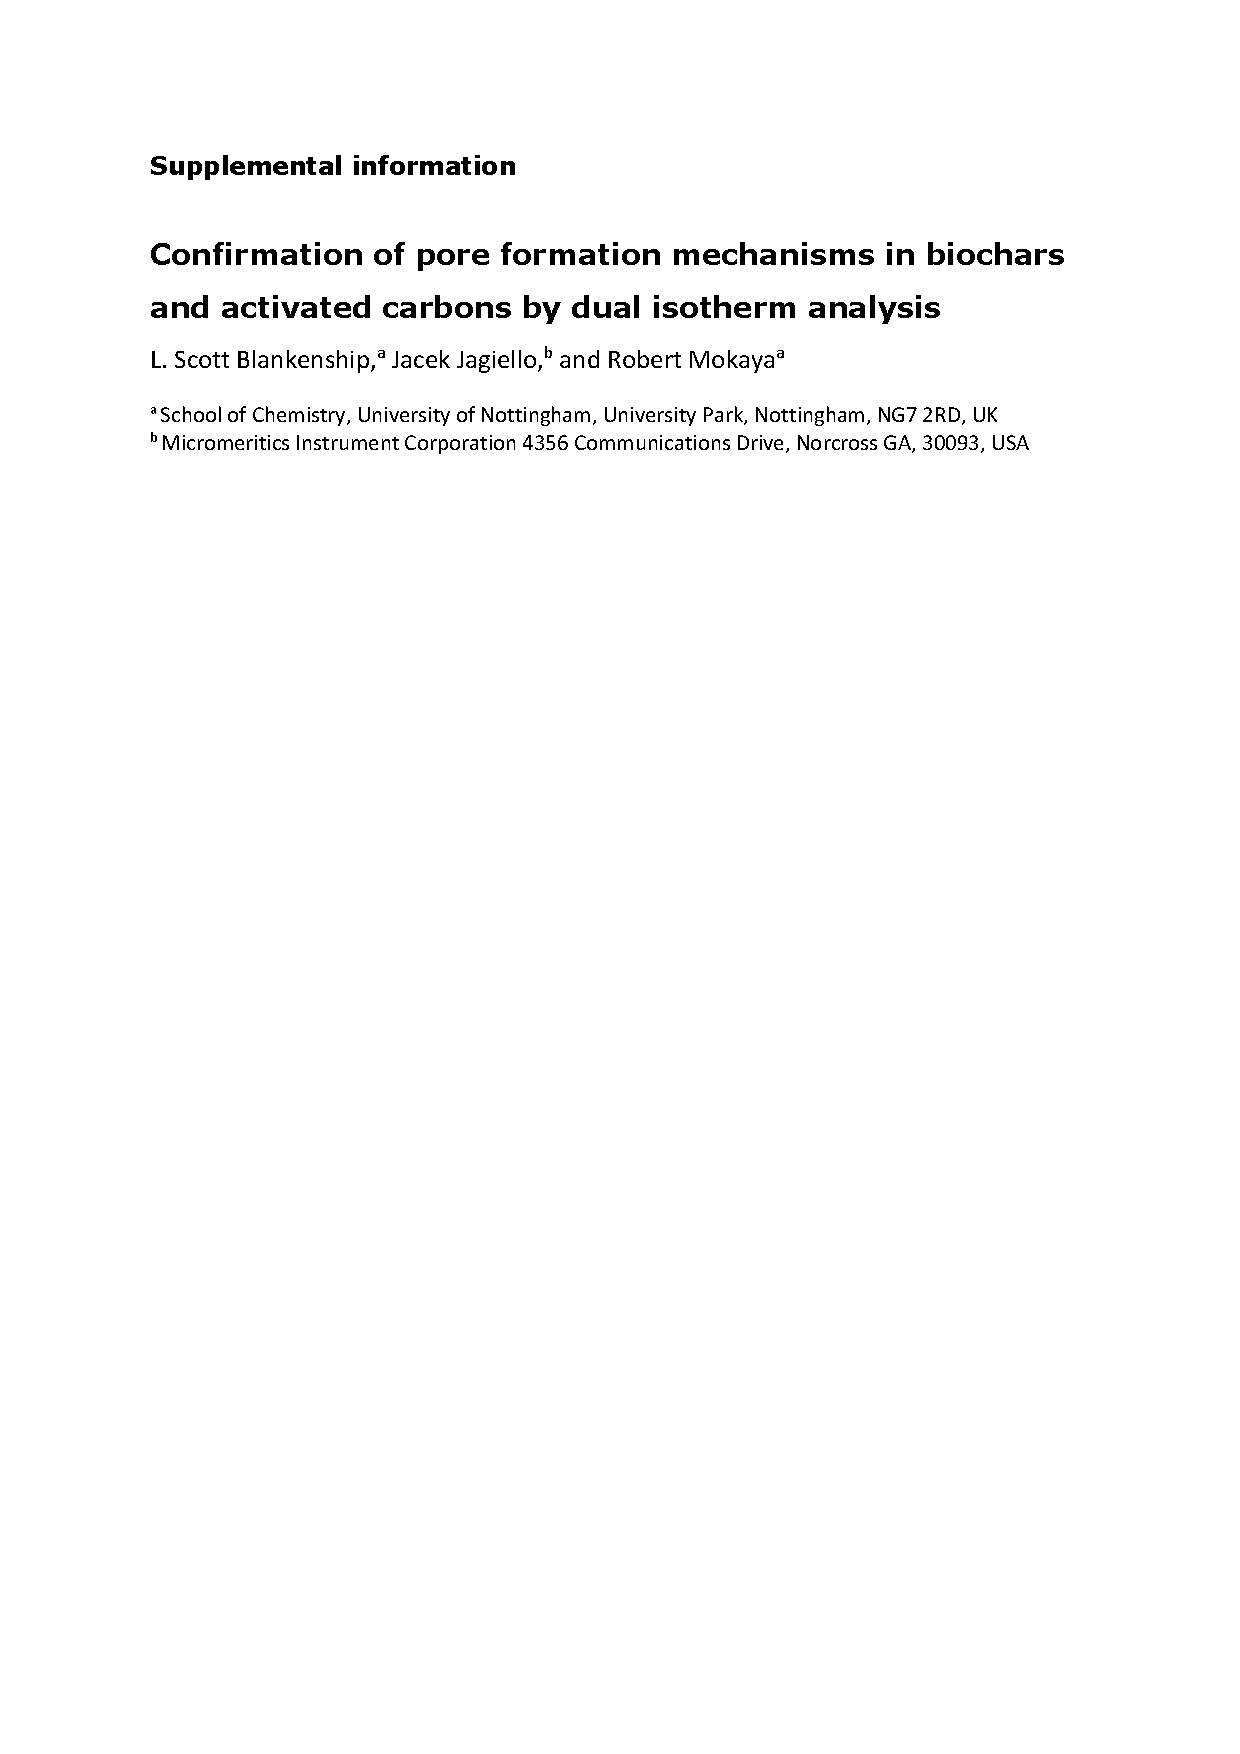
\includepdf[pages=-]{si_02}
\setlength{\voffset}{\originalVOffset}
\setlength{\hoffset}{\originalHOffset}



\section*{References}